\chapter{Modeling}

The modeling phase is divided into three Business Objectives (BO), each addressing a specific aspect of breast cancer diagnosis and prognosis. This chapter details the mathematical formulations, hyperparameter choices, and business ("métier") rationale for the selected models.

\section{Business Objective 1: Tumor Classification (Diagnostic)}
The primary goal of BO1 is to accurately classify tumor samples as \textbf{Benign} or \textbf{Malignant} based on cytological features. We developed and optimized three distinct architectures: a Hybrid GRU-SVM model, Softmax Regression, and an SGD-optimized SVM.

\subsection{Model 1: Hybrid GRU-SVM}
To further improve classification performance, particularly in minimizing False Negatives, we implemented a hybrid architecture combining Deep Learning for feature extraction with a traditional SVM classifier.

\subsubsection{Concept}
Standard models treat features as independent or linearly related. This hybrid model uses a \textbf{Gated Recurrent Unit (GRU)} to learn complex, non-linear latent representations of the data, which are then fed into an \textbf{SVM} for the final decision. This leverages the feature learning capability of Neural Networks and the max-margin robustness of SVMs.

\subsubsection{Mathematical Formulation}
\begin{itemize}
    \item \textbf{Feature Reshaping:} The 30 input features are reshaped into a sequence $X \in \mathbb{R}^{5 \times 6}$ (5 timesteps, 6 features per step) to simulate sequential dependency.
    \item \textbf{Feature Extraction (GRU):} The GRU computes a hidden state $h_t$ at each step:
    \[ z_t = \sigma(W_z x_t + U_z h_{t-1}) \]
    \[ r_t = \sigma(W_r x_t + U_r h_{t-1}) \]
    \[ \tilde{h}_t = \tanh(W_h x_t + U_h (r_t \odot h_{t-1})) \]
    \[ h_t = (1 - z_t) \odot h_{t-1} + z_t \odot \tilde{h}_t \]
    The final state is projected to a latent space $L$ via a Dense layer with ReLU activation:
    \[ L = \text{ReLU}(W_L h_T + b_L) \]
    \item \textbf{Classification (SVM):} The latent vector $L$ serves as input to the SVM:
    \[ f(L) = \text{sign}\left(\sum_{i} \alpha_i y_i K(L_i, L) + b\right) \]
\end{itemize}

\subsubsection{Hyperparameter Choice}
\begin{itemize}
    \item \textbf{GRU Structure:} 128 Units, Dropout = 0.5 to prevent overfitting.
    \item \textbf{Learning Rate:} 0.001 for the GRU pre-training.
    \item \textbf{SVM Classifier:} Linear Kernel with a calibrated threshold of 0.25.
\end{itemize}

\subsubsection{Métier Rationale}
\begin{itemize}
    \item \textbf{Latent Feature Discovery:} The GRU acts as a sophisticated "filter," transforming raw cytological measurements into a more separable "latent" representation. This helps in distinguishing cases that look similar in the original space but are biologically different.
    \item \textbf{Sensitivity Focus:} By explicitly monitoring "Missed Cases" (False Negatives), this complex architecture aims to capture subtle patterns of malignancy that simpler linear models might miss, providing a "safety net" for the diagnostic process.
\end{itemize}

\subsection{Model 2: Softmax Regression (Logistic Regression)}
Softmax Regression (or Logistic Regression for binary tasks) models the probability that a sample belongs to the Malignant class.

\subsubsection{Mathematical Formulation}
The hypothesis function applies the sigmoid activation to the linear output:
\begin{equation}
    P(y=1|X) = \sigma(z) = \frac{1}{1 + e^{-(\theta^T X + b)}}
\end{equation}
The model minimizes the Log-Loss (Cross-Entropy) cost function with L2 regularization:
\begin{equation}
    J(\theta) = - \frac{1}{m} \sum_{i=1}^{m} [y^{(i)}\log(\hat{y}^{(i)}) + (1-y^{(i)})\log(1-\hat{y}^{(i)})] + \frac{1}{C} ||\theta||^2
\end{equation}

\subsubsection{Hyperparameter Choice}
We performed a Grid Search to identify the best configuration:
\begin{itemize}
    \item \textbf{Solver:} 'lbfgs' (Limited-memory BFGS) for efficient convergence on small datasets.
    \item \textbf{Regularization (C):} $C=10.0$. A higher $C$ implies weaker regularization, allowing the model to fit the decision boundary more closely to the training data, which is appropriate given the high dimensionality (30 features) relative to sample size.
    \item \textbf{Max Iterations:} 3000 to ensure convergence.
    \item \textbf{Decision Threshold:} $0.477$. This threshold was calibrated to optimize the Sensitivity/Specificity balance.
\end{itemize}

\subsubsection{Métier Rationale}
\begin{itemize}
    \item \textbf{Probabilistic Output:} Unlike simple linear classifiers, this model provides a calibrated probability score. A probability of 99\% vs 51\% allows oncologists to gauge the certainty of the diagnosis.
    \item \textbf{Threshold Calibration:} The threshold was lowered from the default 0.5 to 0.477. In a medical context, this slight bias towards the positive class (Malignant) acts as a safety buffer to reduce False Negatives.
\end{itemize}

\subsection{Model 3: SGD-SVM (Stochastic Gradient Descent)}
The third model employs a Support Vector Machine optimized via Stochastic Gradient Descent (SGD), designed for efficiency and fine-grained control over the learning process.

\subsubsection{Mathematical Formulation}
The model minimizes the regularized Hinge Loss function:
\begin{equation}
    J(w,b) = \frac{1}{n} \sum_{i=1}^{n} L(y_i, f(x_i)) + \alpha R(w)
\end{equation}
where $L$ is the Hinge Loss:
\begin{equation}
    L(y, f(x)) = \max(0, 1 - y(w \cdot x + b))
\end{equation}
The weights are updated iteratively:
\begin{equation}
    w \leftarrow w - \eta \left( \alpha w - \mathbb{I}[y_i(w \cdot x_i + b) < 1] y_i x_i \right)
\end{equation}

\subsubsection{Hyperparameter Choice}
\begin{itemize}
    \item \textbf{Loss Function:} 'hinge' (Standard SVM loss).
    \item \textbf{Penalty:} 'l2' (Ridge regularization).
    \item \textbf{Alpha (Regularization):} Dynamic $\alpha = \frac{1}{5 \times n\_samples}$. This dynamic setting scales regularization with dataset size.
    \item \textbf{Class Weight:} 'balanced'. This automatically adjusts weights inversely proportional to class frequencies, addressing the natural imbalance between Benign and Malignant cases.
    \item \textbf{Learning Rate:} Constant with $\eta_0 = 0.001$.
\end{itemize}

\subsubsection{Métier Rationale}
\begin{itemize}
    \item \textbf{Imbalance Handling:} The \texttt{class\_weight='balanced'} parameter is crucial in oncology, where malignant cases might be fewer than benign ones (or vice versa). It ensures the model doesn't bias towards the majority class.
    \item \textbf{Dynamic Regularization:} The dynamic alpha allows the model to adapt its complexity control based on the sample size, providing a robust solution that scales well if more patient data is collected over time.
\end{itemize}

\section{Business Objective 2: Intelligent Triage \& Resource Allocation}
The second objective addresses the operational bottleneck in radiology departments. We designed an AI-powered triage system to prioritize patient cases based on the predicted probability of malignancy, moving from a "First-In-First-Out" workflow to a Risk-Based Queue.

\subsection{Step 1: Probability Calibration}
To enable granular risk assessment, we require not just a binary label (0/1) but a calibrated probability score $P(y=1|X) \in [0, 1]$.

\subsubsection{Selected Engine}
We utilized the \textbf{SGD-SVM (Calibrated)} model as the core scoring engine. This choice is grounded in the model evaluation and comparison detailed in the next section. Although SVMs typically output a non-probabilistic decision function, we applied \textbf{Platt Scaling (Sigmoid Calibration)} to map the distance from the hyperplane to a probability distribution.

\begin{itemize}
    \item \textbf{Input:} 30 Standardized Nuclei Features.
    \item \textbf{Calibration Method:} Sigmoid function fitting on the validation set.
    \item \textbf{Output:} A continuous risk score where 0\% indicates high certainty of benignity and 100\% indicates high certainty of malignancy.
\end{itemize}

\subsection{Step 2: Explainability (XAI)}
Trust is the primary barrier to AI adoption in healthcare. To bridge this gap, we implemented a dual-layer explainability framework.

\subsubsection{Global Interpretability (Top Drivers)}
We analyzed the model's coefficients to identify which morphological features most strongly influence the cancer prediction. This global explainability was achieved by analyzing the \textbf{Feature Coefficients} from the trained SGD-SVM model.

Figure \ref{fig:feature_importance} visualizes the top drivers, separating "Malignant Drivers" (Positive Coefficients, Red) and "Benign Drivers" (Negative Coefficients, Blue).

\begin{figure}[h]
    \centering
    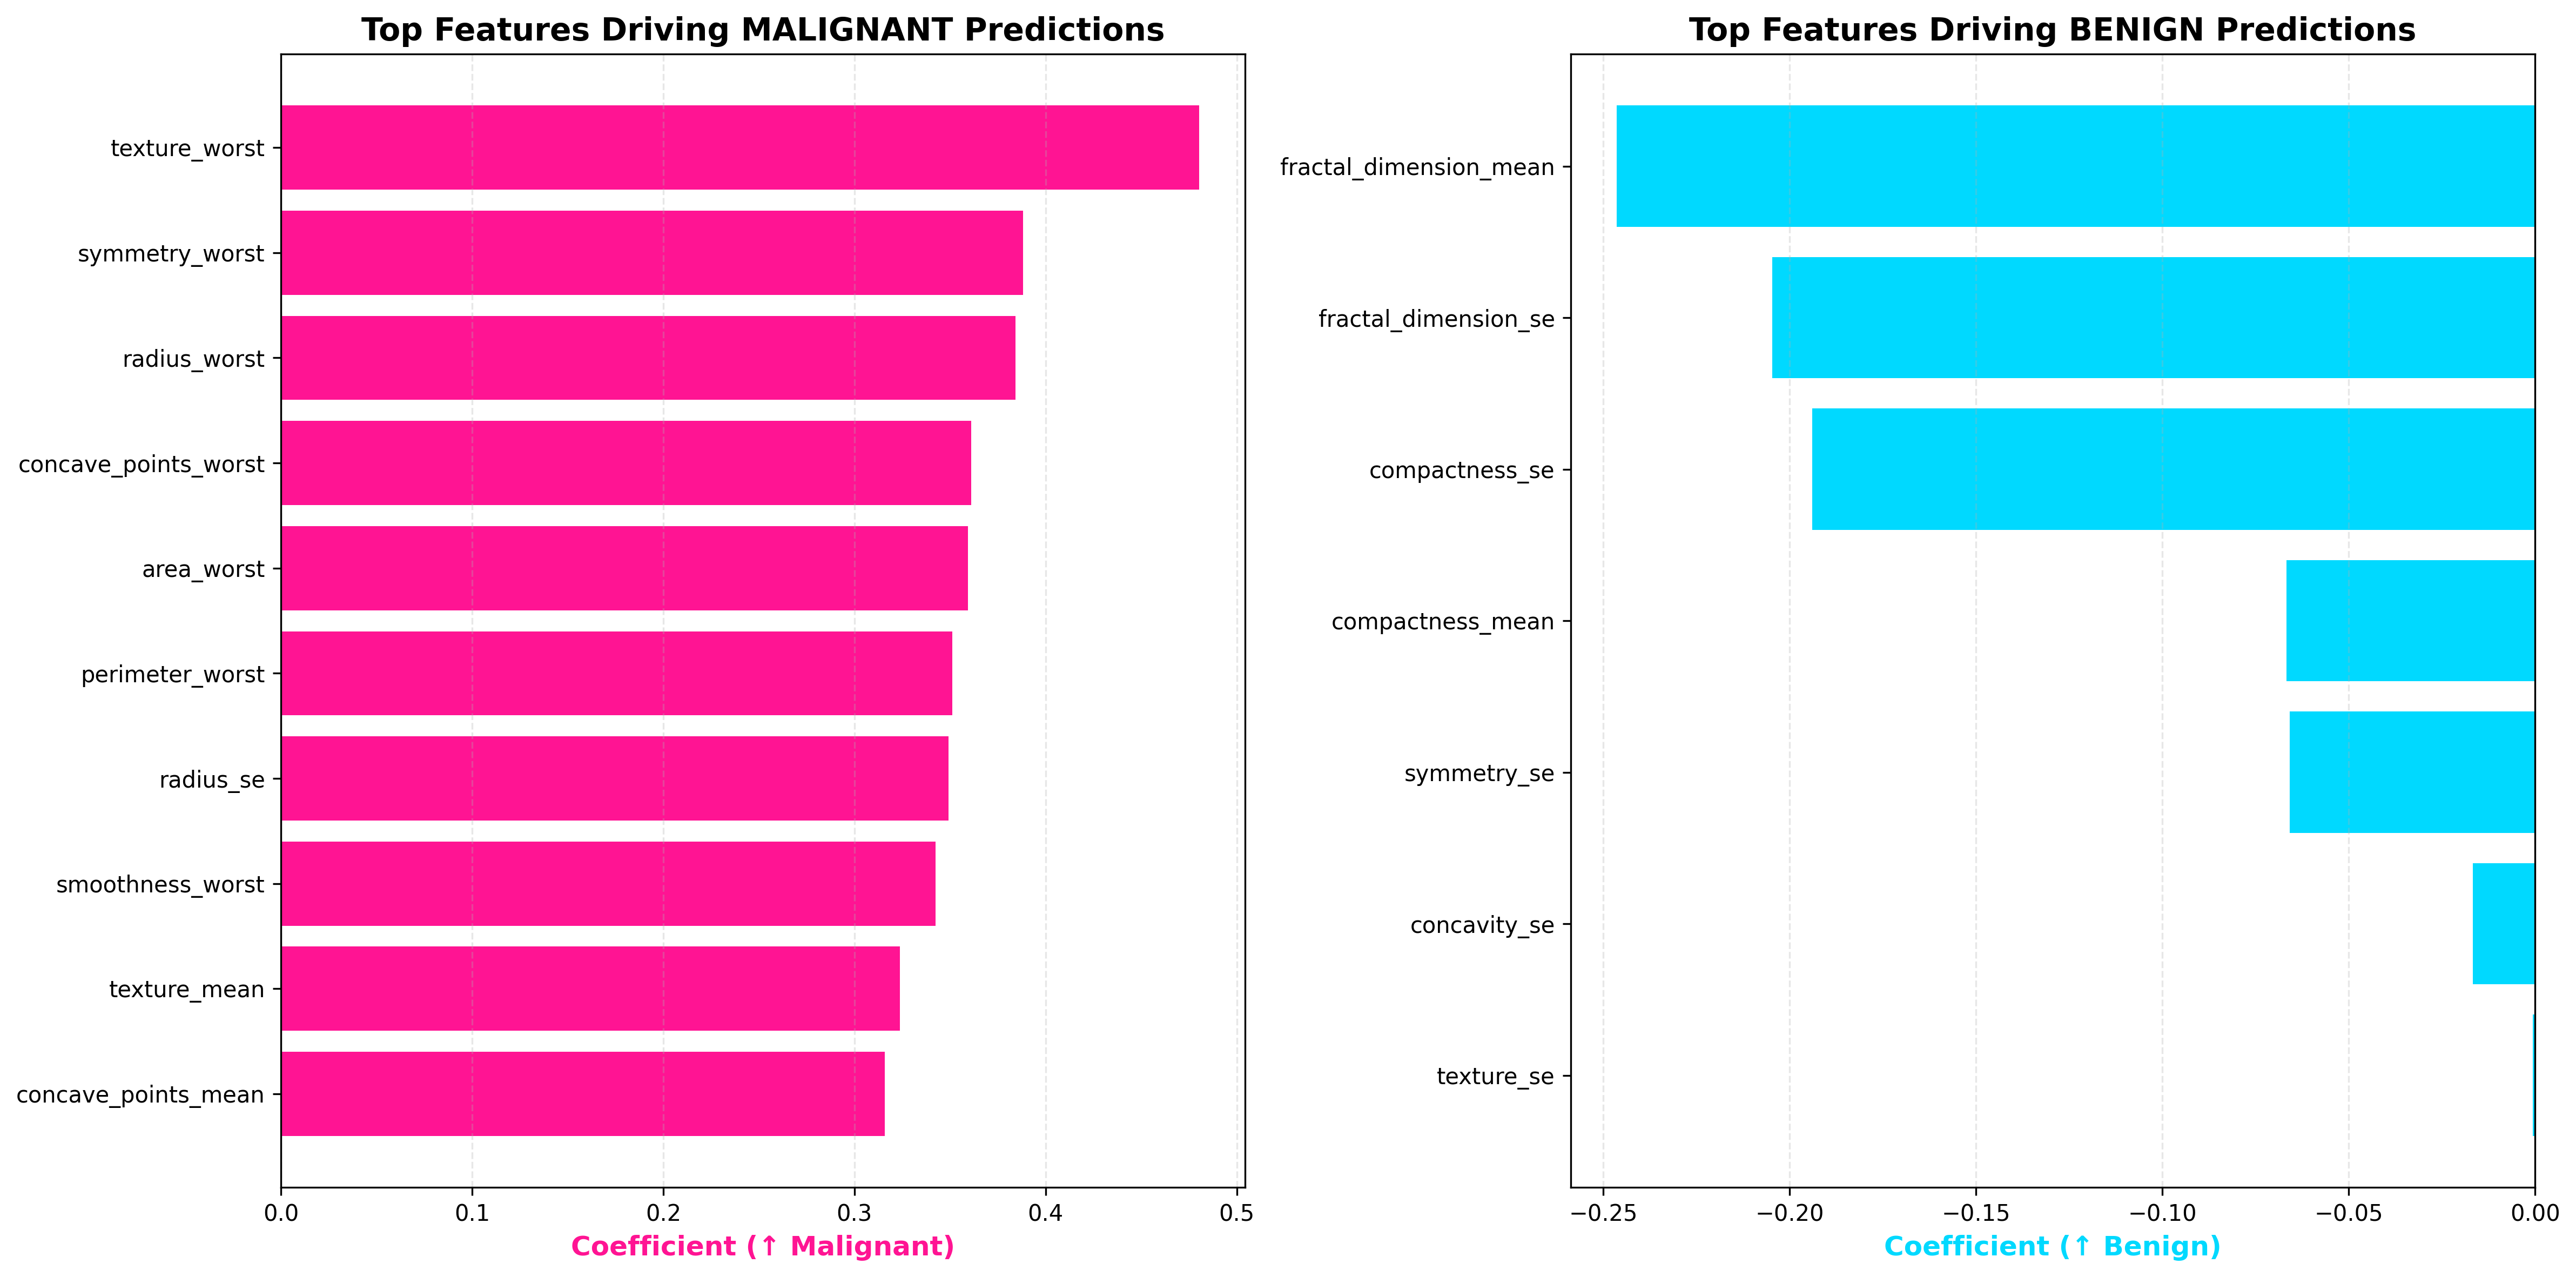
\includegraphics[width=1.0\textwidth]{images/feature_importance_drivers.png}
    \caption{Top Feature Drivers: Malignant (Left) vs Benign (Right)}
    \label{fig:feature_importance}
\end{figure}

The table below summarizes the top drivers identified in our analysis:

\begin{table}[h]
\centering
\begin{tabular}{|l|r|l|}
\hline
\textbf{Feature Name} & \textbf{Coeff} & \textbf{Clinical Significance} \\ \hline
\texttt{texture\_worst} & \textbf{+0.48} & High surface texture variation; indicates structural heterogeneity. \\ \hline
\texttt{symmetry\_worst} & \textbf{+0.39} & Significant cell asymmetry; common in aggressive malignant cells. \\ \hline
\texttt{radius\_worst} & \textbf{+0.38} & Large tumor size; strongly associated with invasive growth. \\ \hline
\texttt{fractal\_dimension\_mean} & \textbf{-0.25} & Driver for benign prediction in this multivariate model. \\ \hline
\texttt{compactness\_se} & \textbf{-0.19} & Driver for benign prediction (lower shape variability). \\ \hline
\end{tabular}
\caption{Top Predictive Drivers and Clinical Interpretation}
\end{table}

\subsubsection{Local Interpretability (SHAP Waterfall)}
To build trust with clinicians, the system provides a detailed "why" for every prediction. We utilize a linear approximation of SHAP values to decompose the model's decision for individual patients.

Figure \ref{fig:shap_waterfall} illustrates the decision path for a high-risk patient (\textbf{Patient P-1461}), who was classified as \textbf{CRITICAL} with a probability of $>99.9\%$.

\begin{figure}[h]
    \centering
    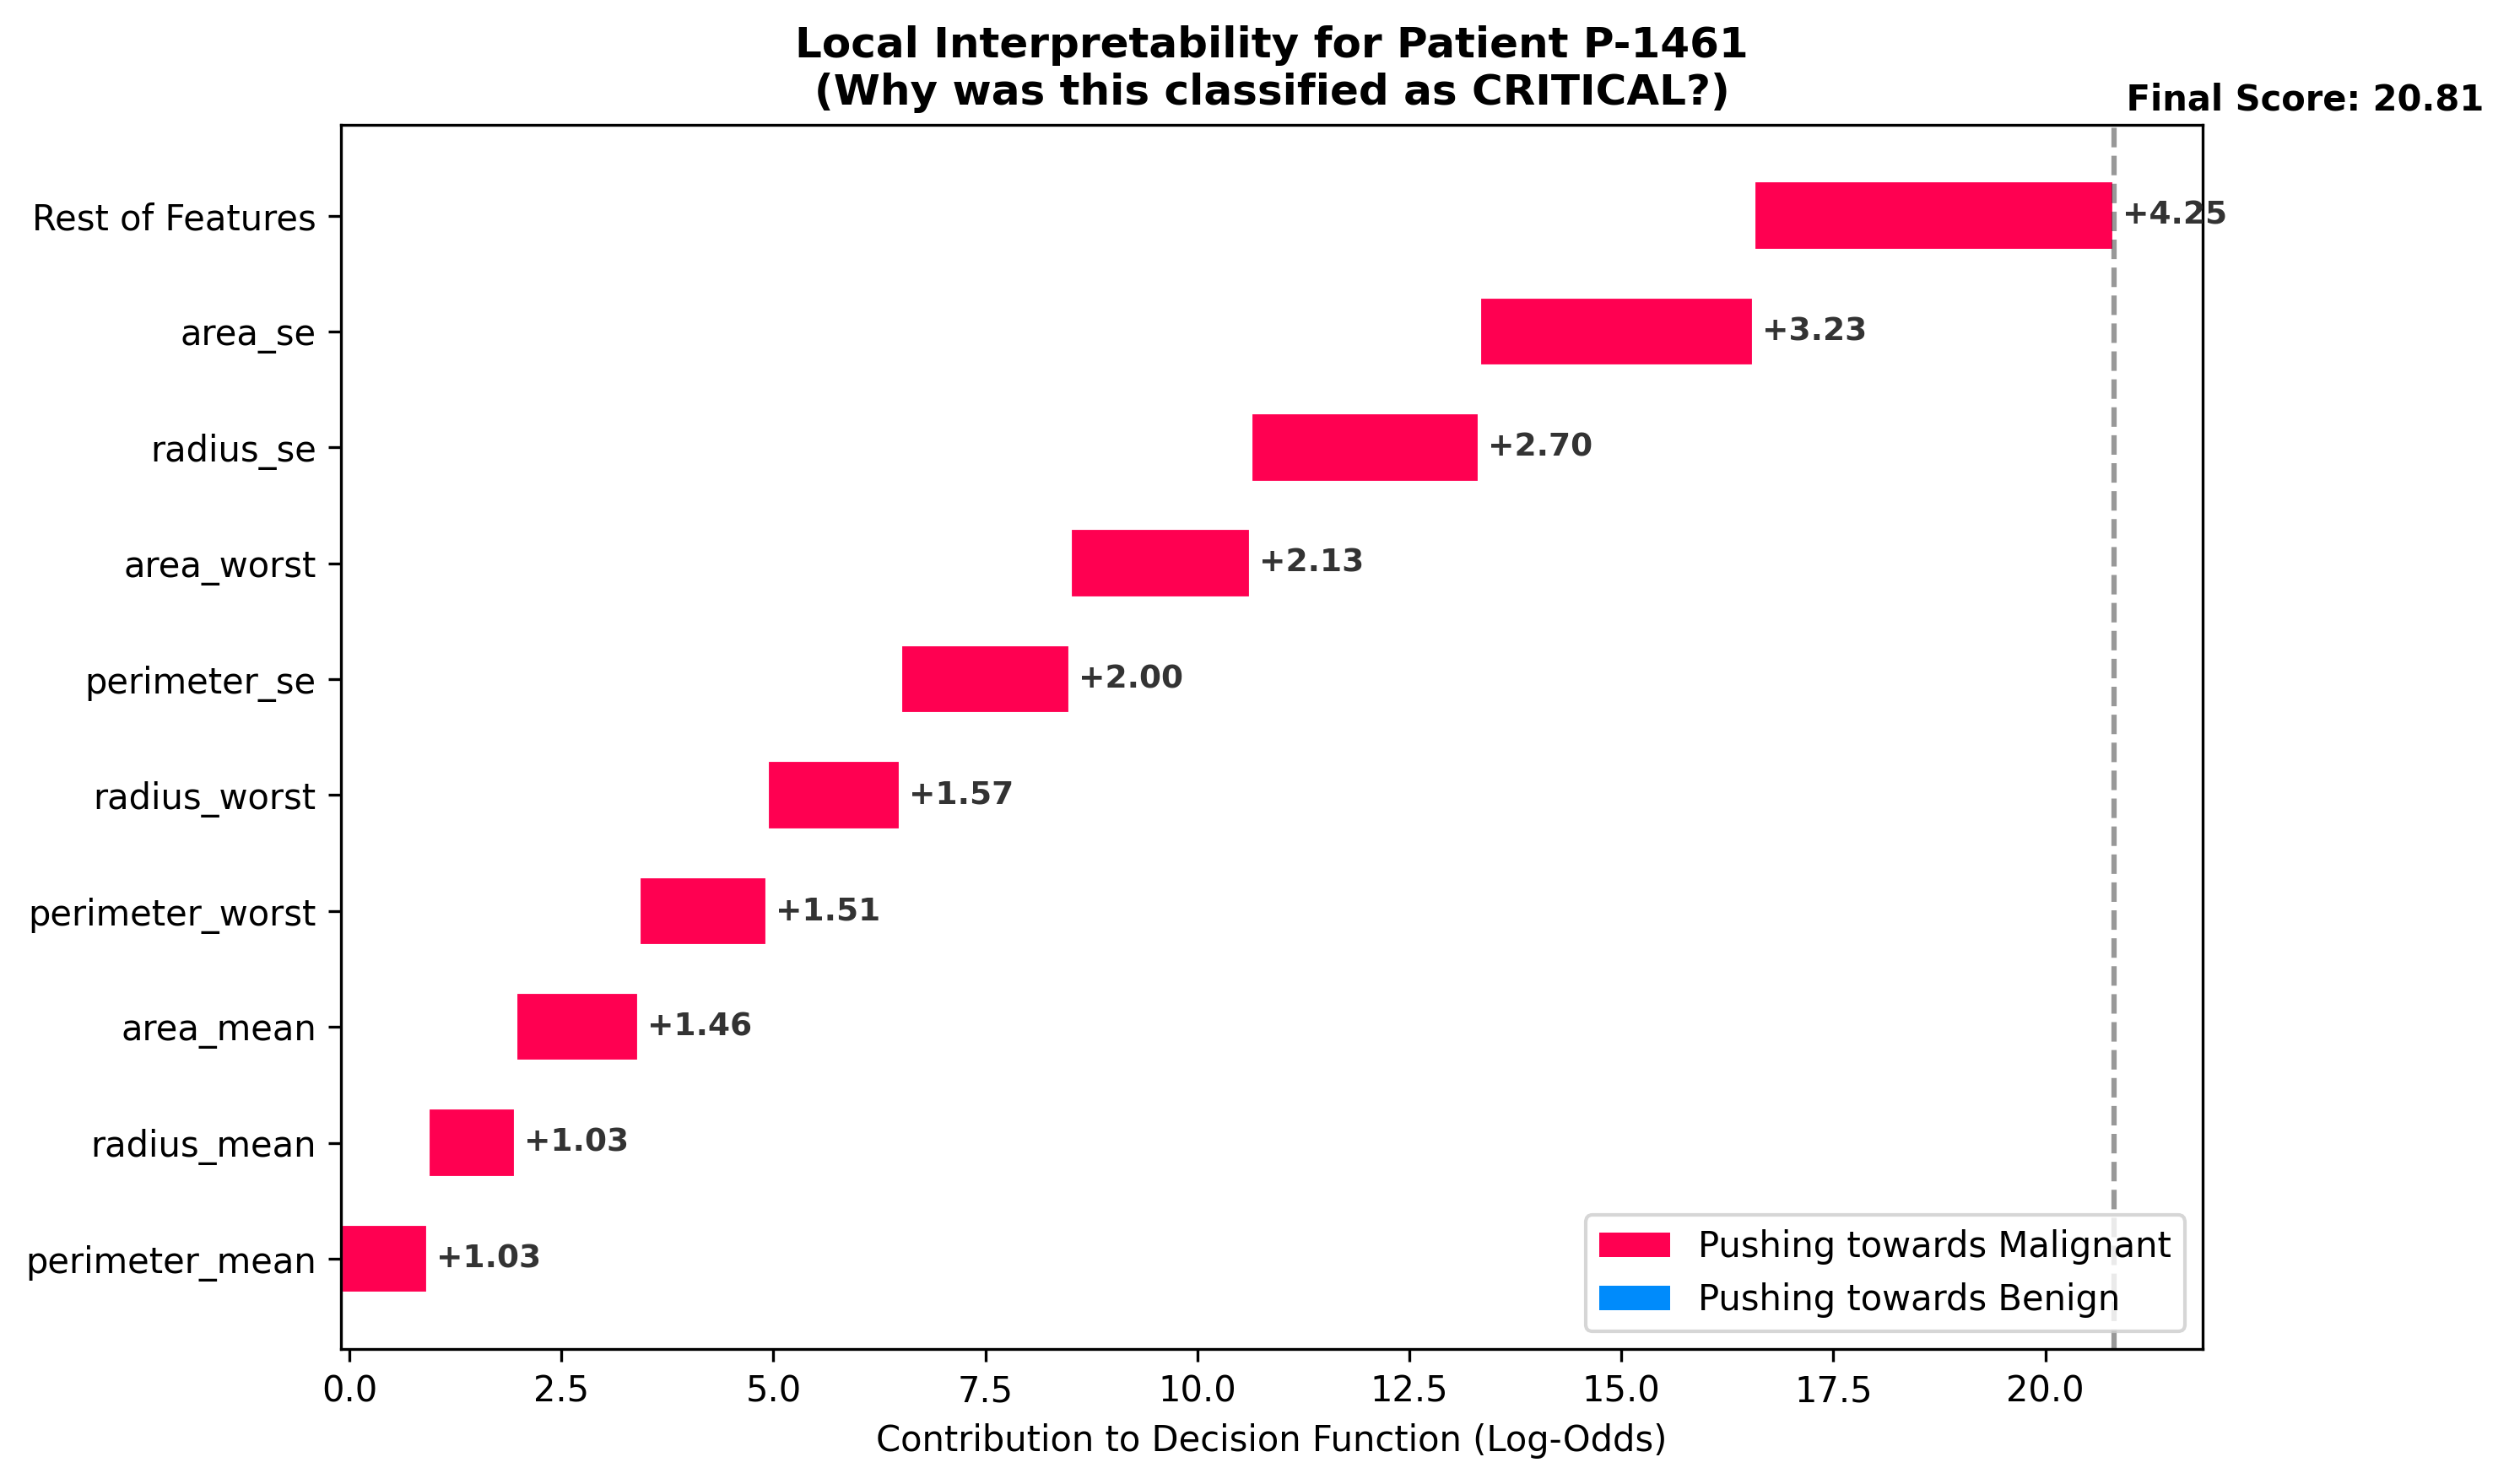
\includegraphics[width=0.9\textwidth]{images/shap_waterfall.png}
    \caption{SHAP Waterfall Plot for Patient P-1461 (Critical Risk)}
    \label{fig:shap_waterfall}
\end{figure}

\textbf{Interpretation of the Graphic:}
\begin{itemize}
    \item \textbf{Base Value:} The starting point is the model's average bias (intercept).
    \item \textbf{\textcolor{red}{Red Bars (Risk Drivers):}} Represent features that push the prediction towards \textit{Malignancy}. For Patient P-1461, the \texttt{texture\_worst} and \texttt{concave\_points\_worst} are significantly elevated, adding substantial weight to the positive class score.
    \item \textbf{\textcolor{blue}{Blue Bars (Protective Factors):}} Represent features that push towards \textit{Benignity}. In this case, their influence is minimal compared to the strong malignant drivers.
    \item \textbf{Final Score:} The cumulative sum results in a high positive log-odds score, which translates to a near-certainty of cancer after sigmoid calibration.
\end{itemize}

This granular view allows radiologists to verify if the AI's "attention" aligns with visible features in the mammogram or biopsy slide (e.g., confirming irregular texture or cell asymmetry).

\subsection{DSO 2.3: Risk Stratification Logic}
\label{sec:risk_stratification}
The system employs a hybrid decision-making model integrating statistical predictions with clinical safety nets:

\begin{itemize}
    \item \textbf{Statistical Stratification:} Patients are categorized into five risk levels (Very Low to Critical) based on calibrated probabilities, guiding specific interventions.
    \item \textbf{Clinical Safety Net:} "Danger Flags" are triggered when physiological features breach safety thresholds.
    \item \textbf{Dynamic Escalation:} Patients with $\ge$ 2 danger flags are automatically upgraded to the next risk tier.
    \item \textbf{Enhanced Prioritization:} A "Priority Queue" flags high-acuity cases ($\ge$ 80\% probability or multiple flags) to ensure immediate attention.
\end{itemize}

\subsubsection{Statistical Risk Stratification}
The table below details the probability thresholds and corresponding clinical actions for each risk tier:

\begin{table}[h]
\centering
\begin{tabular}{|l|l|l|}
\hline
\textbf{Risk Level} & \textbf{Probability Range} & \textbf{Clinical Action} \\ \hline
\textbf{\textcolor{red}{CRITICAL}} & $P \ge 90\%$ & Immediate Biopsy (24-48h) \\ \hline
\textbf{\textcolor{orange}{HIGH}} & $80\% \le P < 90\%$ & Diagnostic Imaging (7 days) \\ \hline
\textbf{\textcolor{yellow}{MEDIUM}} & $40\% \le P < 80\%$ & 6-Month Follow-up \\ \hline
\textbf{\textcolor{green}{LOW}} & $20\% \le P < 40\%$ & Routine Screening \\ \hline
\textbf{VERY LOW} & $P < 20\%$ & Normal Standard of Care \\ \hline
\end{tabular}
\caption{Risk Tiers and Intervention Protocols}
\label{tab:risk_tiers}
\end{table}

\subsubsection{Clinical Safety Net (Danger Flags)}
To prevent false negatives in borderline cases, we monitor specific physiological markers. A "Danger Flag" is raised if a feature exceeds a safety threshold derived from the 90th percentile of malignant cases.

\begin{table}[h]
\centering
\begin{tabular}{|l|c|l|}
\hline
\textbf{Variable} & \textbf{Risk Threshold} & \textbf{Interpretation} \\ \hline
\texttt{texture\_worst} & $> 38.03$ & High surface variation (Danger) \\ \hline
\texttt{radius\_se} & $> 1.00$ & Rapid growth rate indicator (Danger) \\ \hline
\texttt{symmetry\_worst} & $> 0.42$ & High cell asymmetry (Danger) \\ \hline
\texttt{concave\_points\_mean} & $> 0.15$ & Deep indentations (Danger) \\ \hline
\texttt{concavity\_worst} & $> 0.71$ & Severe contour irregularities (Danger) \\ \hline
\end{tabular}
\caption{Danger Flag Thresholds for Dynamic Escalation}
\label{tab:danger_flags}
\end{table}

\textbf{Dynamic Escalation Logic:} If a patient has $\ge$ 2 Danger Flags, their Risk Tier is automatically upgraded (e.g., from \textbf{MEDIUM} to \textbf{HIGH}), ensuring that subtle but dangerous physiological signs are not missed by the statistical model alone.

\subsubsection{Resource Allocation Impact}
This stratified approach allows the hospital to move from a FIFO (First-In-First-Out) queue to a \textbf{Priority Queue}**, ensuring that critical resources (biopsy slots, radiologist time) are allocated to the patients who need them most urgently (The top $\approx$10-20\% of cases).

\section{Business Objective 3: Prognosis \& Evolution (METABRIC)}
The third objective moves beyond diagnosis to \textbf{prognosis}, aiming to predict the future trajectory of the disease. Using the METABRIC genomic dataset, we target three key indicators of tumor progression to answer the question: \textit{"How fast will this tumor grow?"}

\subsection{Target Variables}
\begin{itemize}
    \item \textbf{Aggressiveness Score (0-10):} A composite continuous index derived from tumor grade, size, and lymph node status.
    \item \textbf{Growth Rate (mm/year):} The estimated velocity of tumor expansion.
    \item \textbf{Evolution 6M (Classification):} The predicted clinical status at 6 months:
    \begin{itemize}
        \item \textbf{0 (Stable):} No significant change.
        \item \textbf{1 (Moderate):} Noticeable growth requiring attention.
        \item \textbf{2 (Rapid):} Aggressive expansion requiring immediate intervention.
    \end{itemize}
\end{itemize}

\subsection{Model Architecture \& Configuration}
To handle these diverse targets simultaneously (Regression + Classification-proxy), we employed \textbf{Multi-Output Regression} wrappers around powerful ensemble estimators. We explicitly defined and compared two architectures:

\subsubsection{Selected Models}
The following models were configured to balance bias and variance, using the \texttt{MultiOutputRegressor} wrapper to predict all three targets ($y_{aggr}, y_{growth}, y_{evol}$) simultaneously:

\begin{itemize}
    \item \textbf{Random Forest (Bagging):}
    \begin{itemize}
        \item \textbf{Base Estimator:} \texttt{RandomForestRegressor}
        \item \textbf{Configuration:}
        \begin{itemize}
            \item \texttt{n\_estimators=200}: We doubled the default number of trees to maximize variance reduction (averaging effect).
            \item \texttt{max\_depth=10}: Constraining depth prevents the trees from memorizing noise in the high-dimensional genomic data.
            \item \texttt{n\_jobs=-1}: Utilizes all CPU cores for parallel training.
        \end{itemize}
    \end{itemize}

    \item \textbf{Gradient Boosting (Boosting):}
    \begin{itemize}
        \item \textbf{Base Estimator:} \texttt{GradientBoostingRegressor}
        \item \textbf{Configuration:}
        \begin{itemize}
            \item \texttt{n\_estimators=200}: Ensures the model has enough iterations to correct the residuals of previous trees.
            \item \texttt{learning\_rate=0.1}: A standard learning rate that balances convergence speed with robustness.
            \item \texttt{max\_depth=5}: We use shallower trees compared to Random Forest, as boosting relies on "weak learners" to iteratively reduce bias.
        \end{itemize}
    \end{itemize}
\end{itemize}

\subsubsection{Mathematical Formulation}

\paragraph{Multi-Output Strategy:}
Since standard regressors ($f: X \to y$) typically predict a single scalar, the Multi-Output strategy fits one regressor per target variable. For a target vector $Y = [y_{\text{aggr}}, y_{\text{growth}}, y_{\text{evol}}]$, the model learns three independent functions sharing the same input feature space $X$:
\[ F(X) = \begin{bmatrix} f_1(X) \\ f_2(X) \\ f_3(X) \end{bmatrix} \]
This allows for specific optimization of each task (e.g., minimizing MSE for growth rate) while maintaining a unified pipeline.

\subsection{Métier Interpretability Choices}
\begin{itemize}
    \item \textbf{Non-Linearity:} Tumor growth is rarely linear. Gradient Boosting captures complex interactions between genes and clinical factors (e.g., Age + HER2 status) that simpler linear models would miss.
    \item \textbf{Multi-Faceted Prognosis:} By predicting three distinct targets, we provide a holistic view for the oncologist:
    \begin{itemize}
        \item \textit{Aggressiveness:} "How bad is it now?" (Current State)
        \item \textit{Growth Rate:} "How fast is it changing?" (Velocity)
        \item \textit{Evolution:} "What is the clinical category?" (Triage Class)
    \end{itemize}
    \item \textbf{Interpretability:} Tree-based models allow us to extract "Feature Importance," identifying which specific genes drive the prognosis. This moves the model from a "Black Box" to a "Biomarker Discovery" tool.
\end{itemize}
